Pour rappel, le prototype est constitué des composants suivants :

\begin{itemize}
  \item Raspberry Pi 2B (plateforme)
  \item XL4015 (step-down)
  \item SIM800L (modem)
  \item Carte SIM Thingstream
  \item Circuit imprimé permettant de connecter le Raspberry Pi et le SIM800L
  \item	Un boîtier (avec ou sans ventilateur)
\end{itemize}

\noindent
En plus du matériel requis pour le prototype, les composants suivants sont également nécessaires afin de réaliser le test :

\begin{itemize}
  \item Un Raspberry Pi connecté à Internet (le modèle n’a pas d’importance)
  \item Deux capteurs de température de type DS18B20
  \item Une résistance de $4,7 k\Omega$
\end{itemize}

\noindent
Afin de mieux distinguer les deux Raspberry Pi, le Raspberry Pi 2B sera désormais nommé client. Le Raspberry Pi connecté à Internet sera appelé serveur.

~

\noindent
Avant de démarrer le test, il faut connecter les capteurs de température au serveur. La figure illustre comment effectuer ce branchement.

\begin{figure}
  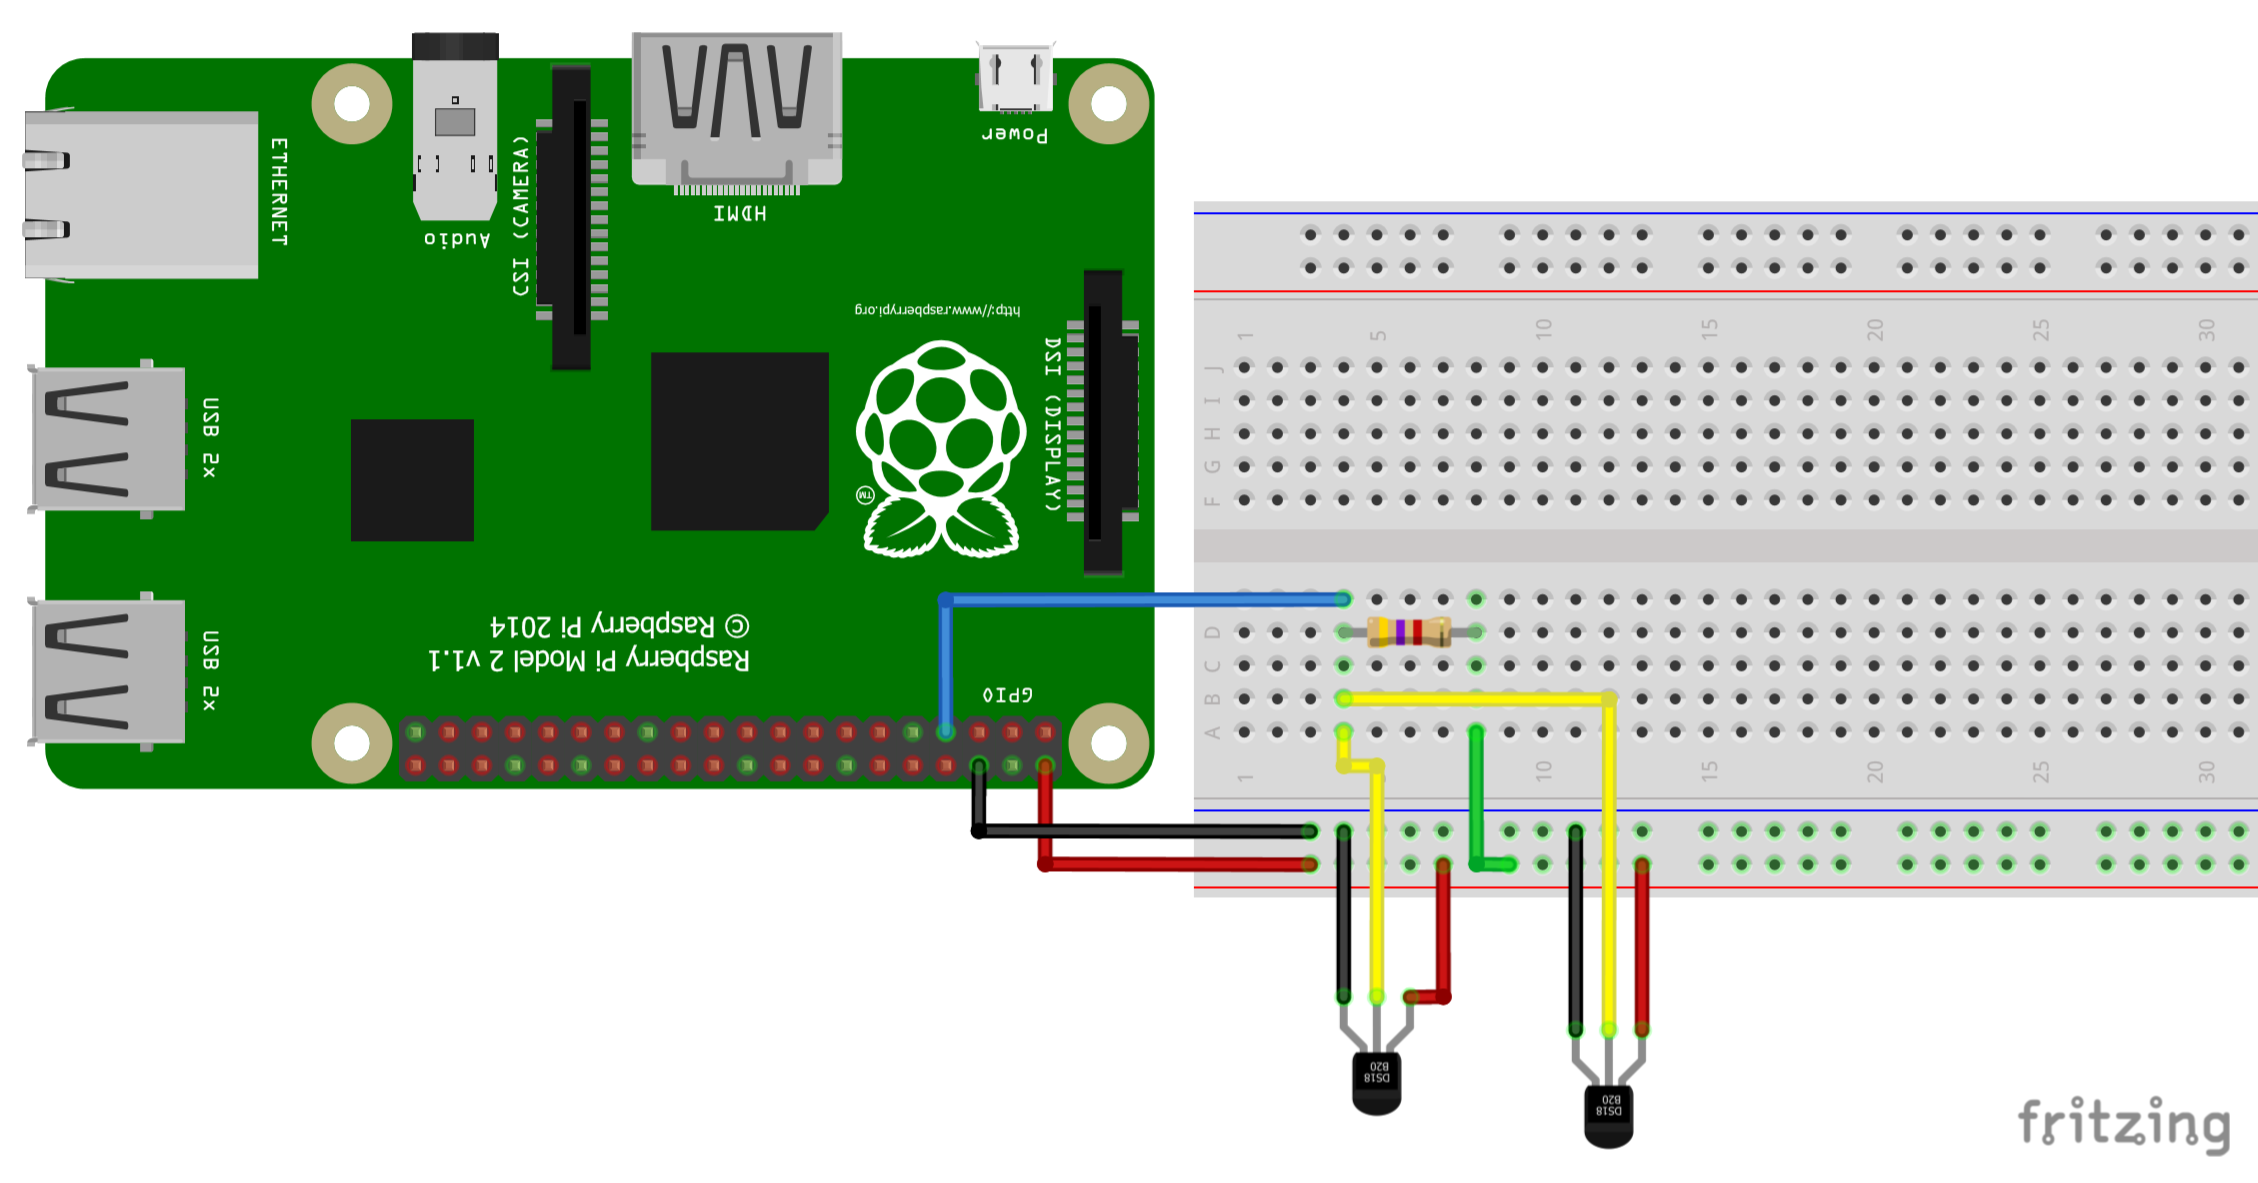
\includegraphics[width=\textwidth]{img/el_prototype/test_conn.png}
  \caption{Schéma des connexions des capteurs de température au Raspberry serveur}
  \label{fig:connnn}
\end{figure}

\noindent
Le premier capteur de température doit être placé à environ 1 cm au-dessus du circuit imprimé qui est placé sur le client. Le deuxième capteur de température doit être placé à plus ou moins 1cm au-dessus du XL4015. La figure 4.2 illustre les régions où les capteurs doivent être placés.

~

\noindent
Ensuite, les scripts python doivent être copiés sur le serveur et le client si cela n’a pas encore été fait. Pour ce faire, vous pouvez utiliser le client SFTP de votre choix. Les fichiers \textit{automated\_test.py}, \textit{client\_test.py}, \textit{cpu\_temp.py} et \textit{MA2\_Communication\_server.jar} doivent être copiés sur le client. Le fichier \textit{server\_test.py} doit être copié sur le serveur. Sur ce dernier fichier, veuillez configurer les variables \textit{CLIENT\_ID}, \textit{USERNAME} et \textit{PASSWORD} avec des paramètres permettant de se connecter à la plateforme de Thingstream. (Ces valeurs se trouvent sur votre portail de Thingstream)

~

\noindent
Pour lancer le test du côté du client, seulement le programme dans \textit{automated\_test.py} doit être exécuté. Ce programme se chargera de lancer tous les autres programmes requis pour le test. Cependant, pour lancer le programme, les paramètres suivants doivent être passés en argument lors de l’exécution :

\begin{itemize}
  \item -r $[int]$ : durée totale du test en seconds
  \item -t $[int]$ : temps en seconds entre chaque mesure de la température du CPU
  \item -m $[int]$ : temps en seconds entre la publication de chaque message
  \item -f $[str]$ : nom du fichier avec les résultats
\end{itemize}

~

\noindent
De façon similaire, plusieurs paramètres sont requis pour exécuter le \textit{serser\_test.py}. Les arguments sont les suivants :

\begin{itemize}
  \item -r $[int]$ : durée totale du test en seconds
  \item -t $[int]$ : temps en seconds entre chaque mesure prise pas les capteurs DS18B20
  \item -f $[str]$ : nom du fichier avec les résultats
\end{itemize}

~

\noindent
Le protocole de test peut être divisé en deux parties. La première partie a comme durée la valeur passée avec le paramètre r moins 900 seconds. Les 15 dernières minutes (900 seconds) correspondent à la deuxième partie du test. Cette première partie est composée par la succession d’étapes suivantes.

\begin{enumerate}
  \item Deux cœurs du CPU du client sont soumis à un stress test. Ce stress test se prolonge pendant toute la première partie du protocole de test.
  \item En parallèle, le prototype publie un message sur le topic \textit{device/\{identity\}/post} toutes les -m secondes. Après avoir publié son message, le client attend pendant 2 minutes maximum une réponse du serveur.
  \item Le serveur reçoit le message publié par le client et vérifie si ce message est valide. Le résultat de cette vérification est enregistré sur le fichier avec le nom du paramètre -f. Ensuite, le serveur publie une réponse sur le topic \textit{device/\{identity\}/startup}.

  \item Si le client reçoit la réponse du serveur endéans les 2 minutes à la suite de l’envoi du message, alors la réponse du serveur est écrite sur le fichier de nom -f. Dans le cas contraire, un message d’erreur est écrit au lieu du message.

  \item Pendant que les étapes précédentes ont lieu, le client enregistre la température du CPU toutes les -t secondes sur un deuxième fichier de nom "temps\_ + -f".

  \item Pareillement, le serveur enregistre aussi les températures mesurées avec les capteurs de température sur un fichier de nom "temps\_ + -f". Ces mesures sont aussi effectuées toutes les -t secondes.
\end{enumerate}

~

\noindent
Lors des 15 dernières minutes, seulement des mesures de température sont effectuées. Il est ainsi plus facile de comparer la façon dont le boîtier ou les différentes solutions de refroidissement sont capables de libérer la chaleur des différents composants.
Lors de ce mémoire, tous les tests effectués en suivant ce protocole ont été réalisés à l’aide des commandes suivantes :

~

\begin{lstlisting}[language=bash, caption=Commande client]
python3 automated_test.py -r 18000 -t 30 -m 240 -f client_test.txt
\end{lstlisting}


\begin{lstlisting}[language=bash, caption=Commande serveur]
python3 server_test.py -r 18000 -t 30 -f server_test.txt
\end{lstlisting}

~

\noindent
Ceci veut donc dire que les tests avaient une durée de 5 heures, les mesures de température étaient effectuées une fois toutes les 30 secondes et un message était publié par le client une fois toutes les 4 minutes. Les deux commandes doivent être lancées l'une après l'autre sans aucun ordre particulier.
